
\setbeamertemplate{background}
{
\includegraphics[width=\paperwidth,height=\paperheight]{images/ragazze_digitali.jpg}}
\begin{frame}
\end{frame}

\setbeamertemplate{background}{}

\begin{frame}{Alcune regole..}
	\begin{itemize}
	    \item Mano alzata
    \end{itemize}
\end{frame}

\begin{frame}{Alcune regole..}
	\begin{itemize}
	    \item Mano alzata
        \item Si Copia!
    \end{itemize}
\end{frame}

\begin{frame}{Alcune regole..}
	\begin{itemize}
	    \item Mano alzata
        \item Si Copia!
        \item Divertirsi!
    \end{itemize}
\end{frame}

\begin{frame}{Che cos'è la Scienza}
    
\footnote{Traduzione dalle slides del Prof. Andrea Omicini, Sistemi Distribuiti AA 18/19}
\begin{block}{Da: The Science Council}
\small{\url{http://sciencecouncil.org/about-us/our-definition-of-science/}}
% Science  is  the  pursuit  and  application  of  knowledge  and  understanding  of  the  natural  and  social  world  following  a  systematic methodology based on evidence
\vspace{0.5cm}

La Scienza è la ricerca e l'applicazione della conoscenza e della comprensione dei fenomeni naturali e sociali, che avviene seguendo una metodologia sistematica basata sui fatti.
\end{block}

\end{frame}

\begin{frame}{Che cos'è la Scienza}
    
\begin{block}{Da: The Science Council}
\small{\url{http://sciencecouncil.org/about-us/our-definition-of-science/}}
\vspace{0.5cm}

La Scienza è la ricerca e l'applicazione della conoscenza [..] seguendo una metodologia sistematica [...]
% In inglese "informatica" si dice Computer Science, quindi in questa settimana noi saremo scienziati (utilizzando i computer)
\end{block}

\end{frame}

\setbeamertemplate{background}
% Python
{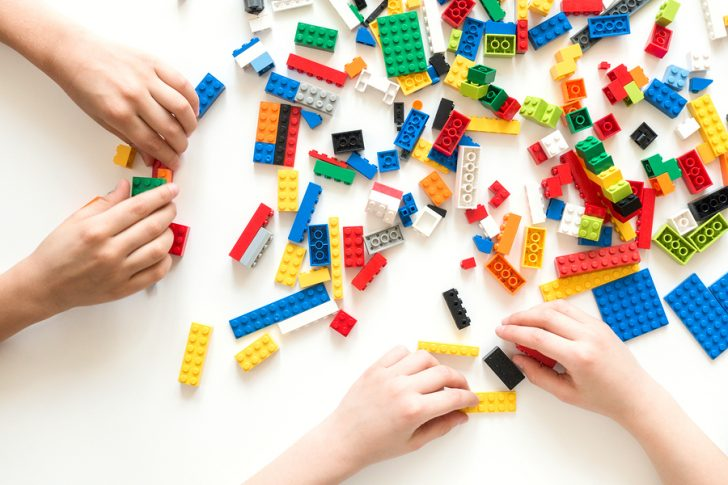
\includegraphics[width=\paperwidth,height=\paperheight]{images/lego.jpg}}
\begin{frame}{Cosa faremo}
\end{frame}

\setbeamertemplate{background}{}

\begin{frame}{Python}
    \begin{block}{Italiano}
        Ciao Mondo!
    \end{block}

    \begin{block}{Inglese}
        Hello World!
    \end{block}

    \begin{block}{Python}
        print "Hello World!"
    \end{block}
    
    \small{Faremo riferimento a questo libro, potete scaricarlo legalmente gratis
    \url{https://inventwithpython.com/invent4thed/}}

\end{frame}

\setbeamertemplate{background}
% Python
{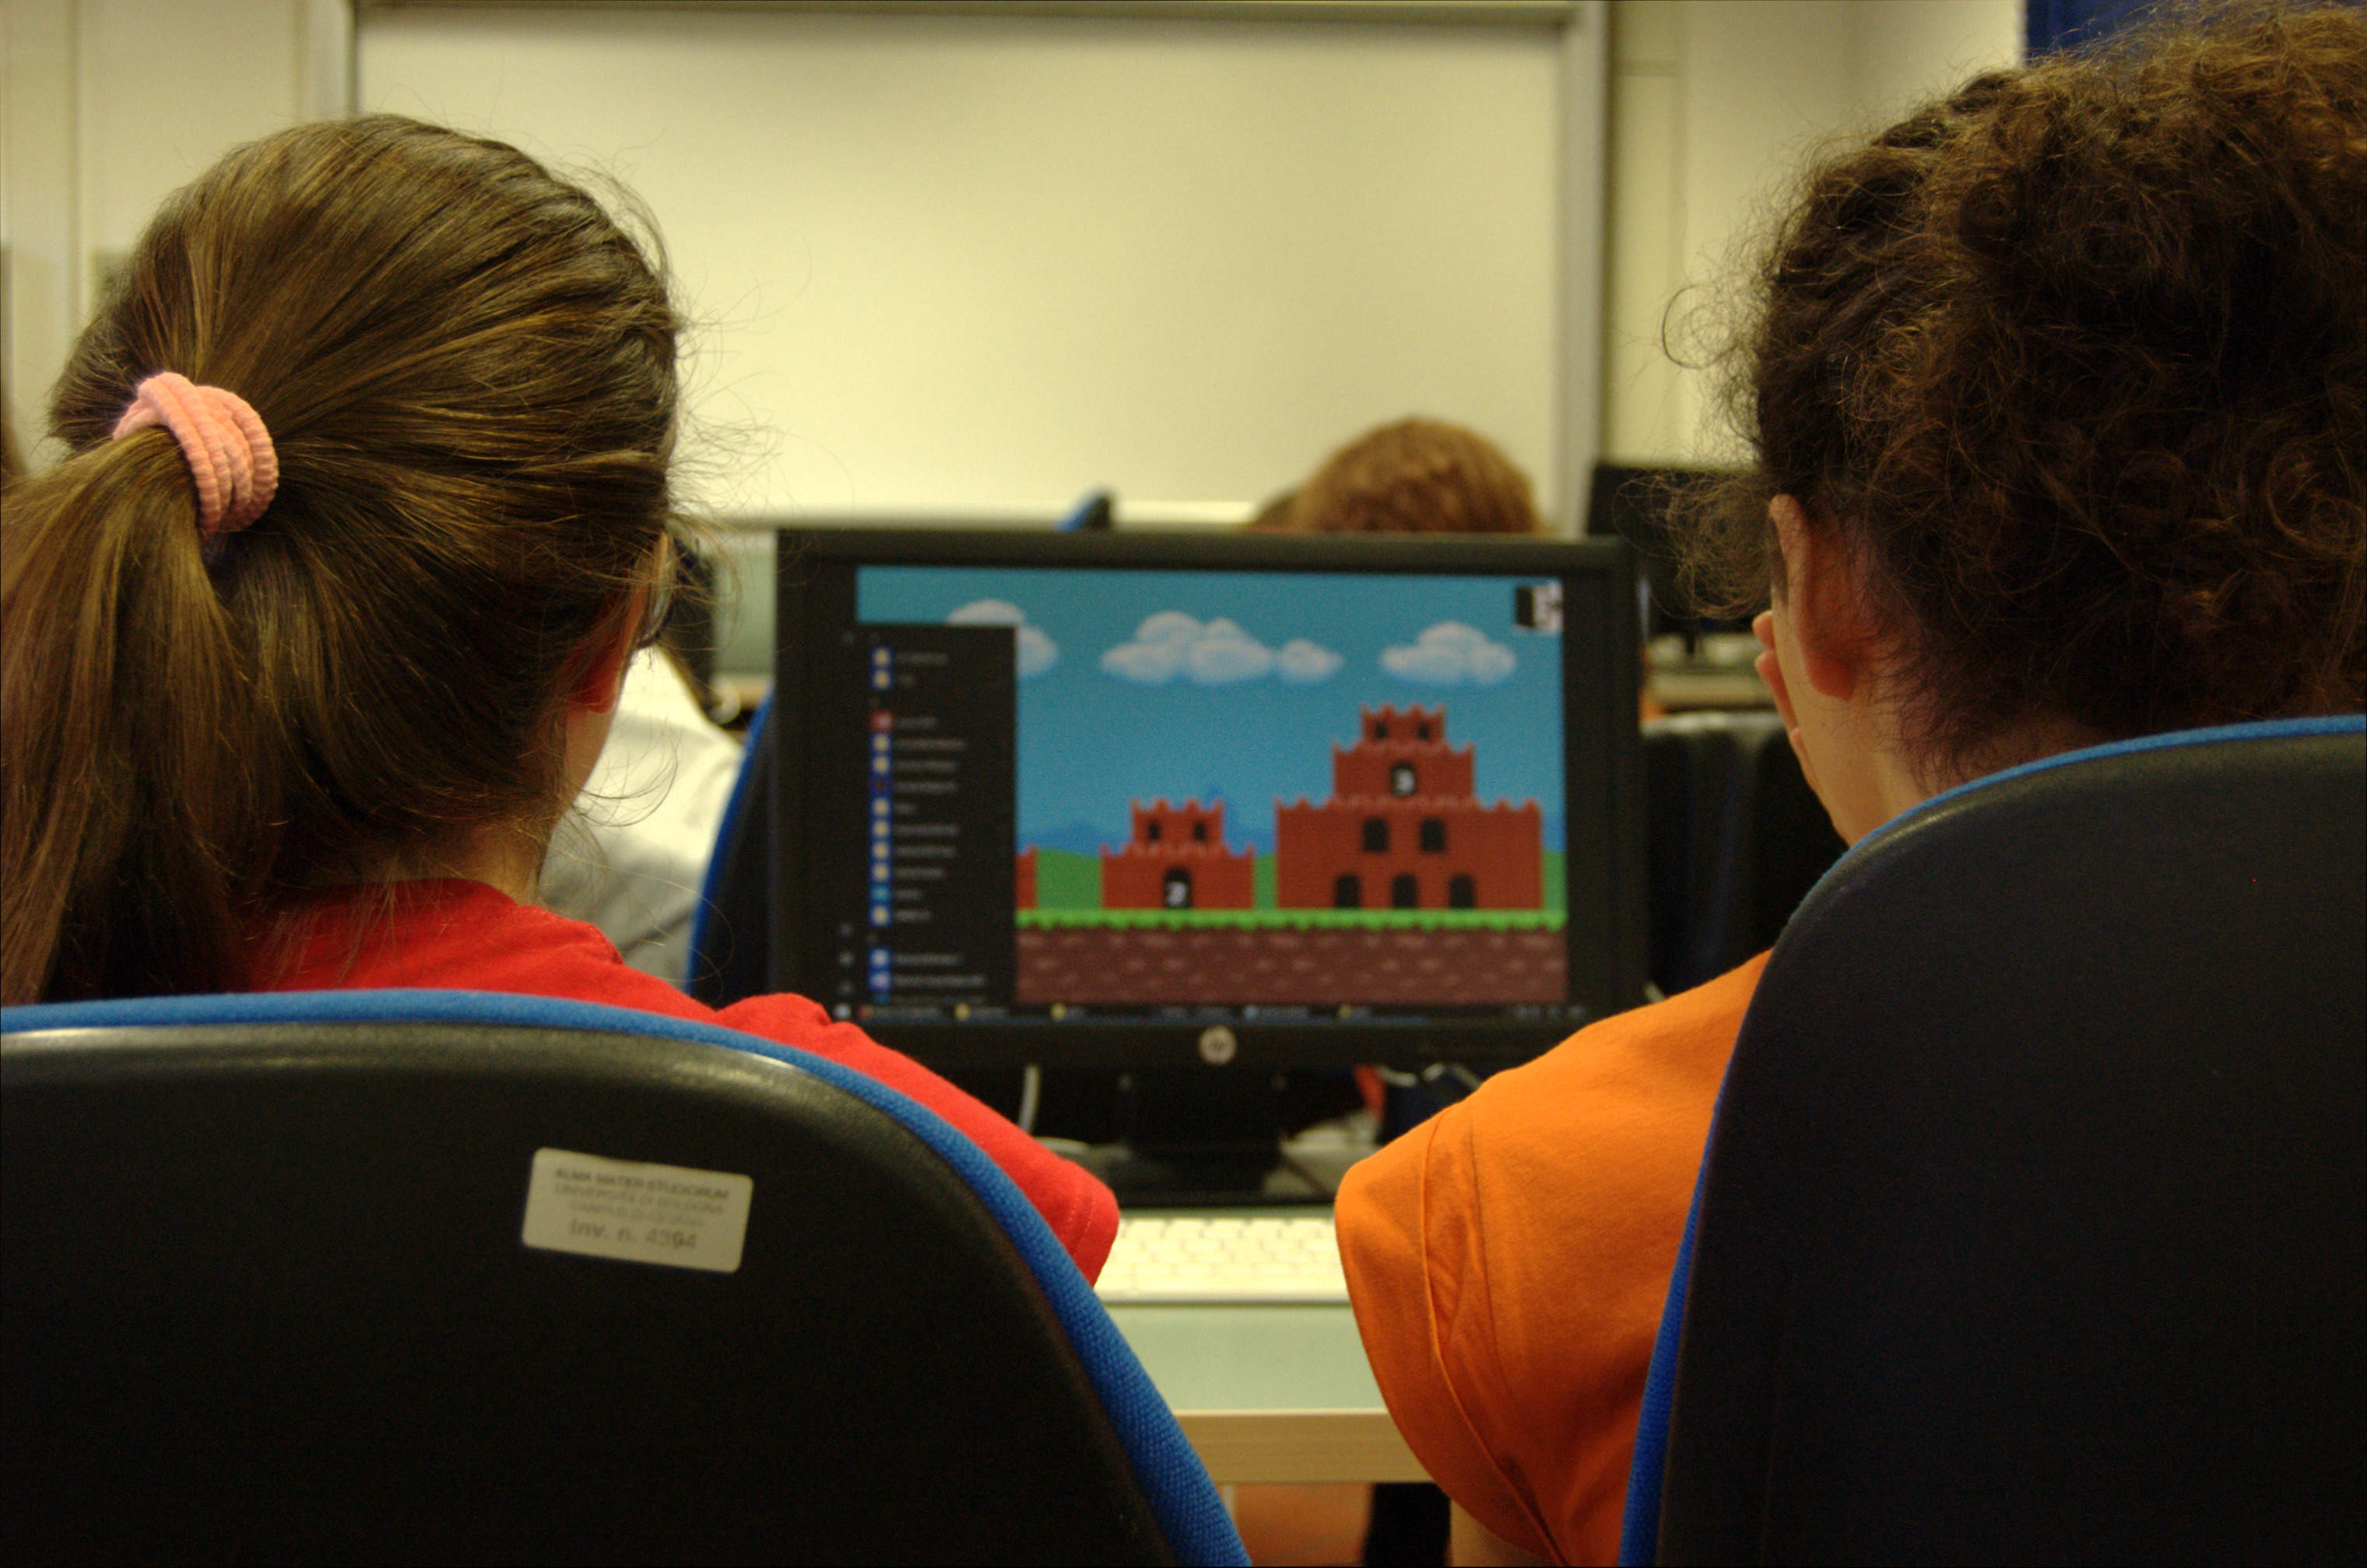
\includegraphics[width=\paperwidth,height=\paperheight]{images/summer_camp_2018_10.jpg}}
\begin{frame}{Cosa faremo}
\end{frame}

\setbeamertemplate{background}
% Python
{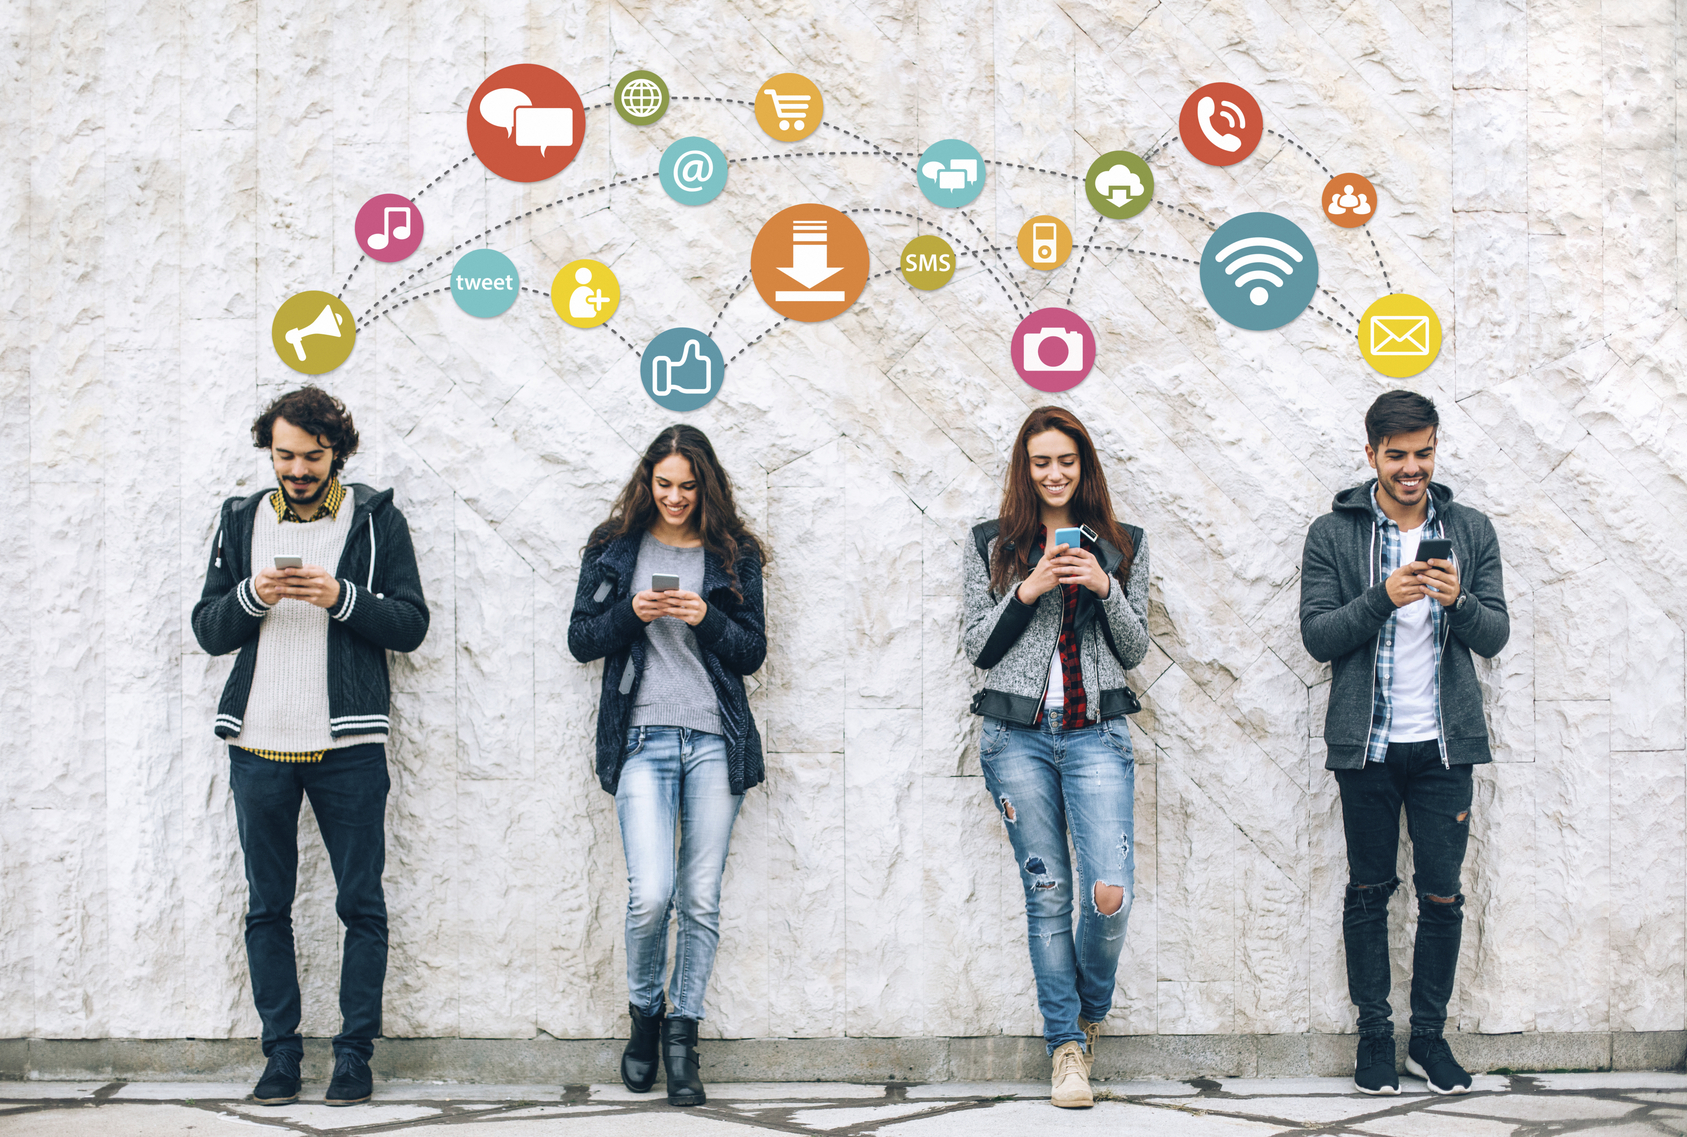
\includegraphics[width=\paperwidth,height=\paperheight]{images/competing_on_social_media.jpg}}
\begin{frame}{Cosa faremo}
    \vspace{0.8cm}
    \begin{block}{Siete Ragazze \textbf{Digitali}!}
      		\begin{itemize}
      		    \item Fake News
    			\item Social Network
    			\item Software Libero
    			\item Sicurezza
    		\end{itemize}
    \end{block}
\end{frame}